\chapter{Technical Appendix}
\label{sec:techappendix}
In this technical appendix, we present an overview of the methodologies employed in our research, regarding GPT's testing phase. This supplementary section aims to provide a transparent and thorough account of the technical aspects for future reproducibility.

\section{Test Execution}
We tested the model capabilities using OpenAI's GPT API with gpt-3.5-turbo, which is the most cost-effective OpenAI model. Entering the testing phase, we had a few key expectations regarding GPT capabilities:
\begin{itemize}
      \item Sentiment Analysis. We aimed to understand if GPT could accurately determine the sentiment (positive, negative, or neutral) in a given text.
      \item Multi-option Question Answering. We aimed to evaluate GPT's ability to extract the necessary information from a text to answer multi-option questions effectively.
      \item Data Extraction. We aimed to explore how well GPT could identify and extract valuable data from both call transcriptions and working notes.
\end{itemize}
Our testing phase focused on assessing GPT's performance in these practical contexts to understand its strengths and weaknesses when applied to competence mapping tasks. Each testing phase has been divided into 4 sub-phases: Preprocess phase, Prompt construction phase, API call phase, and Results analysis phase.
\begin{enumerate}
      \item Preprocess phase. Initially, we prepared the testing data. This phase involved data cleaning and the creation of an input that the model could understand. OpenAI's best practices were followed in terms of spacing and clear distinction between different portions of the text.
      \item Prompt construction phase. During the prompt construction phase, we carefully crafted the instructions and questions intended for the model, adhering to OpenAI's guidelines to optimize the quality and efficacy of the results obtained. We made sure to specify the structure of the answer in an unequivocal way so that the model would answer in a format that allowed us to automatize the testing process.
      \item API call phase. We executed calls by transmitting the prompt to the model through the GPT3.5 API.
      \item Result analysis phase. Upon receiving the model's response, a thorough analysis of the results was conducted, and prompts were adjusted as necessary.
\end{enumerate}

\subsection{Communication competence testing}
We initiated communication competence tests to adhere to OpenAI's guidelines and best practices. The primary objective is to assess operators' ability to effectively engage with customers. We are evaluating factors such as kindness, clarity in explanations, and overall customer satisfaction with the assistance provided. Additionally, we are employing sentiment analysis to understand the emotional tone of customer-operator interactions and gauge how people feel about the support they receive. More in detail:
\begin{itemize}
      \item Kindness. The model was asked to evaluate the kindness of the operator throughout the whole conversation.
      \item Clarity in explanations. The model was tasked with assessing the operator's skill in effectively communicating information or providing explanations for potential solutions to customers' problems. This may involve guiding customers through the steps to resolve their issues or, if needed, explaining the underlying cause along with suggested solutions that the company can implement.
      \item Pitch sale execution. In the \href{https://zenodo.org/records/4274454}{I-BiDaaS TID Synthetic Call Centre Dataset}, we observed that the actor portraying the operator was frequently tasked with promoting a new product to the customer while addressing their request. To assess GPT's capability to discern the presence or absence of this scenario in the provided transcriptions, we aimed to evaluate whether the model could accurately identify instances where customer support operators deviate from established behavioral guidelines. This becomes particularly important in situations where companies have set specific guidelines for their customer support representatives and would want to understand if such guidelines are respected.
      \item Customer satisfaction. The model was asked to understand the general satisfaction of the customer.
\end{itemize}

Various prompt variants were tested, as detailed in the following section (see \ref{sec:testingresults}). In the initial approach, a single question was posed in a single prompt, asking the model to assess the operator's communication competence with a score ranging from 0 to 4. In the second approach, four distinct questions were presented in a single prompt. The model was prompted to evaluate four communication characteristics: Kindness, Ability to explain, Execution of pitch sale, and Customer satisfaction. The first, second, and fourth questions sought a value between 0 and 1 (0, 0.25, 0.5, 0.75, 1), while the third question required a binary response (0 or 1). To ensure the model focused on individual tasks, the third approach involved posing four questions in separate prompts, each requesting a response between 0 and 1 (0, 0.25, 0.5, 0.75, 1). Similarly, in the final approach, four questions were presented in separate prompts, each seeking a binary answer (0 or 1). As mentioned earlier, in response to the absence of negative behavior examples, we augmented the existing dataset by incorporating nine additional transcriptions. Each transcription is a modified version of an existing one in the original dataset, primarily focusing on creating scenarios where the operator exhibited unprofessional behavior during interactions with the customer.

\subsection{Technical competence testing}
\label{sec:techcomp}


One of the competences under evaluation is the operator's proficiency in resolving technical issues. In the case of AEM Fiber, operators are required to categorize each issue into a broad category. Our objective is to task the model with determining if the category selected by the operator aligns with the actual issue based on the ticket description. Additionally, the model is challenged to identify the sub-category associated with the ticket, aiming for a more detailed assessment of the operator's capabilities. This approach recognizes that solving similar issues in different contexts may require different solutions. In our testing, we assessed GPT's ability to accurately identify both the category and subcategory of a ticket using the ticket descriptions from the Milwaukee Dataset, with a provided list of possible categories. To model the category recognition task, where categories are very different, we selected five distinct categories from the Milwaukee Dataset. The considered categories are as follows:
\begin{itemize}
      \item 'Interior of Building in Disrepair'
      \item 'Missed Collection: Garbage'
      \item 'Pothole'
      \item 'Sanitation Inspector Notification'
      \item 'Street Light Out'
\end{itemize}
These selected categories do not overlap in any conceivable manner. To model the subcategory recognition task, we focused on the subcategories related to the "Garbage Cart" issue within the dataset. The objective is to assess the model's ability to identify very similar classes of tickets. To assist GPT in this task, we chose to provide additional information about each subcategory in the prompt. This decision is rooted in the assumption that companies like AEM Fiber possess the capacity to discern the nuances within their services, enabling them to identify the key terms that accurately distinguish each subcategory. The considered sub-categories of Garbage cart are: Additional, Damaged, Delete, and Missing.\\

To evaluate the model's ability to identify elements within the text, we tasked it with recognizing the name of the street where the issue occurred. We manually extracted the location of the problem and compared the model's response with our expected label. For this comparison, we utilized a Python package that measures the distance between two strings. If a certain threshold was surpassed, the answer was deemed correct. The package employs Levenshtein Distance to calculate differences between strings \cite{fuzzywuzzy}. For instance, in the AEM Fiber use case, this approach could prove valuable in identifying details such as the router model and manufacturer. This introduces an additional layer of information about the technical operator's capabilities, considering that different routers require distinct knowledge.

\subsection{Problem management testing}
The ultimate goal here is to evaluate the technician's problem-solving abilities, particularly in managing various client issues, described in helpdesk tickets. The operator is tasked with documenting every step of the problem management process in work notes. In our evaluation, we provided GPT with the work notes related to a ticket without explicitly specifying which ticket they corresponded to. Subsequently, we assessed GPT's capacity to accurately identify if the notes adhered to the guidelines established by domain experts. For example, if a ticket needs to be resolved within two days, we asked GPT to analyze the work notes to determine if the tickets were appropriately resolved within 48 hours. Additionally, considering the significance of keeping the client continuously updated during the ticket resolution process, we tasked GPT with identifying if this requirement was met by the technician. The complete list of requests made to GPT is available in section \ref{sec:probmanageres}. Each question includes a set of possible answers, and we assigned a specific score to each answer. In the initial test phase, we initially asked GPT all these questions in a single call. However, we observed improved performance when each question corresponded to a single query. For each group of notes related to a ticket, we manually determined the expected scores and then compared them with the scores given by GPT.

\section{Testing Results}
\label{sec:testingresults}

We will now provide an example of the structure used for each prompt. Initially, we described to the model the provided text format and content. Occasionally we also told GPT to assume the role of a persona following the OpenAI best practices.
\begin{center}
      \textit{You need to evaluate the following conversation between a customer and an operator, contained in a list. Each sentence in the list is separated by a comma and starts with an identifier that reveals who is speaking (Either 'Customer' or 'Tech'). You are a Human Resources employee and you have to answer the following question:}
\end{center}
We then added a question to the prompt.
\begin{center}
      \textit{Is the number of days it took to resolve the issue greater than 2? Yes: -1; No: +1.}
\end{center}
We also provided the model with examples and additional information regarding each competence and finally we explained to the model which rating scale to use and the answer structure.
\begin{center}
      \textit{Give me 1 if the operator was professional, 0 otherwise. You have to answer only with the score for each question.}
\end{center}
We considered appropriate the choice of the Root Mean Square Error (RMSE) as the metric for measuring GPT's error, especially given its effectiveness in quantifying the accuracy of predictions in regression problems. The RMSE provides a comprehensive evaluation of the differences between predicted and actual values, making it a suitable metric for assessing GPT's performance in this context. Specifically, the RMSE is calculated by computing the difference between the target value \(\hat{y_i}\) and the GPT predicted value \(y_i\).
\begin{center}
      \[ RMSE: \sqrt{ \frac{1}{n}\sum_{i=1}^n (\hat{y_i} - y_i)^2}\]
\end{center}

\section{Communication Results}

\subsection{Version 1.0}
The prompt was structured as described before. The following is the version-specific question:\\

\textit{How good was the communication competence of the tech operator?}\\

The following are the obtained results:\\
\begin{center}
      \begin{tabular}{cccc}
            \toprule
            Transcription number (\#) & Overall (OV) & Target Overall (TOV) & Difference \\
            \midrule
            1                         & 4            & 4                    & 0          \\
            2                         & 4            & 4                    & 0          \\
            3                         & 4            & 4                    & 0          \\
            4                         & 4            & 4                    & 0          \\
            5                         & 4            & 4                    & 0          \\
            6                         & 4            & 3                    & -1         \\
            7                         & 4            & 4                    & 0          \\
            8                         & 4            & 4                    & 0          \\
            9                         & 4            & 4                    & 0          \\
            10                        & 4            & 3                    & -1         \\
            11                        & 2            & 2                    & 0          \\
            12                        & 1            & 0                    & -1         \\
            13                        & 2            & 1                    & -1         \\
            14                        & 1            & 1                    & 0          \\
            15                        & 0            & 0                    & 0          \\
            16                        & 4            & 2                    & -2         \\
            17                        & 1            & 0                    & -1         \\
            18                        & 0            & 0                    & 0          \\
            \bottomrule
      \end{tabular}

\end{center}

\subsection{Version 1.1}
The prompt was structured as described before. The questions are the same as in the previous version. The following are the obtained results:
\begin{center}
      \begin{tabular}{ccccccccccccc}
            \toprule
            \# & KIND & EXP & SALE & SAT & TKIND & TEXP & TSALE & TSAT & OV & TOV & DIFF \\

            \midrule
            1  & 1    & 1   & 1    & 1   & 1     & 1    & 1     & 1    & 4  & 4   & 0    \\
            2  & 1    & 1   & 1    & 1   & 1     & 1    & 1     & 1    & 4  & 4   & 0    \\
            3  & 1    & 1   & 1    & 1   & 1     & 1    & 1     & 1    & 4  & 4   & 0    \\
            4  & 1    & 1   & 1    & 1   & 1     & 1    & 1     & 1    & 4  & 4   & 0    \\
            5  & 1    & 1   & 1    & 1   & 1     & 1    & 1     & 1    & 4  & 4   & 0    \\
            6  & 1    & 1   & 1    & 1   & 1     & 1    & 0     & 1    & 4  & 3   & -1   \\
            7  & 1    & 1   & 1    & 1   & 1     & 1    & 1     & 1    & 4  & 4   & 0    \\
            8  & 1    & 1   & 1    & 1   & 1     & 1    & 1     & 1    & 4  & 4   & 0    \\
            9  & 1    & 1   & 1    & 1   & 1     & 1    & 1     & 1    & 4  & 4   & 0    \\
            10 & 1    & 1   & 0    & 1   & 1     & 1    & 0     & 1    & 3  & 3   & 0    \\
            11 & 0    & 0   & 1    & 0   & 0     & 1    & 1     & 0    & 1  & 2   & 1    \\
            12 & 0    & 0   & 0    & 0   & 0     & 0    & 0     & 0    & 0  & 0   & 0    \\
            13 & 0    & 0   & 0    & 0   & 0     & 0    & 0     & 0    & 0  & 0   & 0    \\
            14 & 0    & 0   & 0    & 0   & 0     & 0    & 0     & 0    & 0  & 0   & 0    \\
            15 & 0    & 0   & 0    & 0   & 0     & 0    & 0     & 0    & 0  & 0   & 0    \\
            16 & 1    & 1   & 1    & 1   & 1     & 1    & 1     & 0    & 4  & 3   & -1   \\
            17 & 0    & 0   & 0    & 0   & 0     & 0    & 0     & 0    & 0  & 0   & 0    \\
            18 & 0    & 0   & 0    & 0   & 0     & 0    & 0     & 0    & 0  & 0   & 0    \\
            \bottomrule
      \end{tabular}
\end{center}

\subsection{Version 2.0}
The prompt was structured as described before. The following are the version specific questions:\\

\textit{Was the tech operator kind?\\
      Was the tech operator able to explain himself?\\
      Was the tech operator able to mention the existence of additional products while conversating with the customer?\\
      Was the customer satisfied with the tech service in the end?
}\\

The following are the obtained results:\\
\begin{center}
      \begin{tabular}{ccccccccccccc}
            \toprule
            \# & KIND & EXP  & SALE & SAT  & TKIND & TEXP & TSALE & TSAT & OV   & TOV  & DIFF  \\
            \midrule
            1  & 0.75 & 1.00 & 1    & 0.75 & 1.00  & 1.00 & 1     & 1.00 & 3.50 & 4.00 & 0.50  \\
            2  & 0.75 & 1.00 & 1    & 1.00 & 1.00  & 0.75 & 1     & 1.00 & 3.75 & 3.75 & 0.00  \\
            3  & 0.75 & 1.00 & 1    & 0.75 & 1.00  & 0.75 & 1     & 1.00 & 3.50 & 3.75 & 0.25  \\
            4  & 0.75 & 1.00 & 1    & 0.75 & 1.00  & 0.75 & 1     & 1.00 & 3.50 & 3.75 & 0.25  \\
            5  & 0.75 & 1.00 & 1    & 0.75 & 1.00  & 1.00 & 1     & 1.00 & 3.50 & 4.00 & 0.50  \\
            6  & 0.75 & 1.00 & 0    & 0.75 & 1.00  & 0.75 & 0     & 0.75 & 2.50 & 2.50 & 0.00  \\
            7  & 0.75 & 0.75 & 1    & 0.75 & 1.00  & 1.00 & 1     & 1.00 & 3.25 & 4.00 & 0.75  \\
            8  & 0.75 & 1.00 & 1    & 0.75 & 1.00  & 1.00 & 1     & 1.00 & 3.50 & 4.00 & 0.50  \\
            9  & 0.75 & 1.00 & 1    & 1.00 & 1.00  & 1.00 & 1     & 1.00 & 3.75 & 4.00 & 0.25  \\
            10 & 0.75 & 0.75 & 0    & 0.75 & 1.00  & 1.00 & 0     & 1.00 & 2.25 & 3.00 & 0.75  \\
            11 & 0.75 & 0.75 & 1    & 0.75 & 0.00  & 1.00 & 1     & 0.00 & 3.25 & 2.00 & -1.25 \\
            12 & 0.75 & 0.75 & 0    & 0.50 & 0.00  & 0.00 & 0     & 0.00 & 2.00 & 0.00 & -2.00 \\
            13 & 0.75 & 0.75 & 0    & 0.75 & 0.00  & 0.50 & 0     & 0.00 & 2.25 & 0.50 & -1.75 \\
            14 & 0.75 & 1.00 & 0    & 0.25 & 0.00  & 0.50 & 0     & 0.00 & 2.00 & 0.50 & -1.50 \\
            15 & 0.00 & 0.00 & 0    & 0.00 & 0.00  & 0.00 & 0     & 0.00 & 0.00 & 0.00 & 0.00  \\
            16 & 0.75 & 1.00 & 0    & 0.75 & 0.75  & 1.00 & 1     & 0.50 & 2.50 & 3.25 & 0.75  \\
            17 & 0.75 & 0.75 & 0    & 0.25 & 0.00  & 0.00 & 0     & 0.00 & 1.75 & 0.00 & -1.75 \\
            18 & 0.00 & 0.25 & 0    & 0.00 & 0.00  & 0.00 & 0     & 0.00 & 0.25 & 0.00 & -0.25 \\
            \bottomrule
      \end{tabular}
\end{center}

\subsection{Version 2.1}
The prompt was structured as described before. The questions are the same as in the previous version. The following are the obtained results:
\begin{center}
      \begin{tabular}{ccccccccccccc}
            \toprule
            \# & KIND & EXP & SALE & SAT & TKIND & TEXP & TSALE & TSAT & OV & TOV  & DIFF  \\

            \midrule
            1  & 1    & 1   & 1    & 1   & 1.00  & 1.00 & 1     & 1.00 & 4  & 4.00 & 0.00  \\
            2  & 1    & 1   & 1    & 1   & 1.00  & 0.75 & 1     & 1.00 & 4  & 3.75 & -0.25 \\
            3  & 1    & 1   & 1    & 1   & 1.00  & 0.75 & 1     & 1.00 & 4  & 3.75 & -0.25 \\
            4  & 1    & 1   & 1    & 1   & 1.00  & 0.75 & 1     & 1.00 & 4  & 3.75 & -0.25 \\
            5  & 1    & 1   & 1    & 1   & 1.00  & 1.00 & 1     & 1.00 & 4  & 4.00 & 0.00  \\
            6  & 1    & 1   & 1    & 1   & 1.00  & 0.75 & 0     & 0.75 & 4  & 2.50 & -1.50 \\
            7  & 1    & 1   & 1    & 1   & 1.00  & 1.00 & 1     & 1.00 & 4  & 4.00 & 0.00  \\
            8  & 1    & 1   & 1    & 1   & 1.00  & 1.00 & 1     & 1.00 & 4  & 4.00 & 0.00  \\
            9  & 1    & 1   & 1    & 1   & 1.00  & 1.00 & 1     & 1.00 & 4  & 4.00 & 0.00  \\
            10 & 1    & 1   & 0    & 1   & 1.00  & 1.00 & 0     & 1.00 & 3  & 3.00 & 0.00  \\
            11 & 1    & 1   & 1    & 1   & 0.00  & 1.00 & 1     & 0.00 & 4  & 2.00 & -2.00 \\
            12 & 0    & 1   & 0    & 1   & 0.00  & 0.00 & 0     & 0.00 & 2  & 0.00 & -2.00 \\
            13 & 1    & 1   & 0    & 1   & 0.00  & 0.50 & 0     & 0.00 & 3  & 0.50 & -2.50 \\
            14 & 0    & 1   & 0    & 1   & 0.00  & 0.50 & 0     & 0.00 & 2  & 0.50 & -1.50 \\
            15 & 0    & 0   & 0    & 0   & 0.00  & 0.00 & 0     & 0.00 & 0  & 0.00 & 0.00  \\
            16 & 1    & 1   & 1    & 1   & 0.75  & 1.00 & 1     & 0.50 & 4  & 3.25 & -0.75 \\
            17 & 0    & 0   & 0    & 0   & 0.00  & 0.00 & 0     & 0.00 & 0  & 0.00 & 0.00  \\
            18 & 0    & 0   & 0    & 0   & 0.00  & 0.00 & 0     & 0.00 & 0  & 0.00 & 0.00  \\
            \bottomrule
      \end{tabular}
\end{center}

\subsection{Communication results comparison}
The RMSE was calculated for each version. Both the overall value and each single indicator have been analyzed.
\begin{center}
      \begin{figure}[ht]
            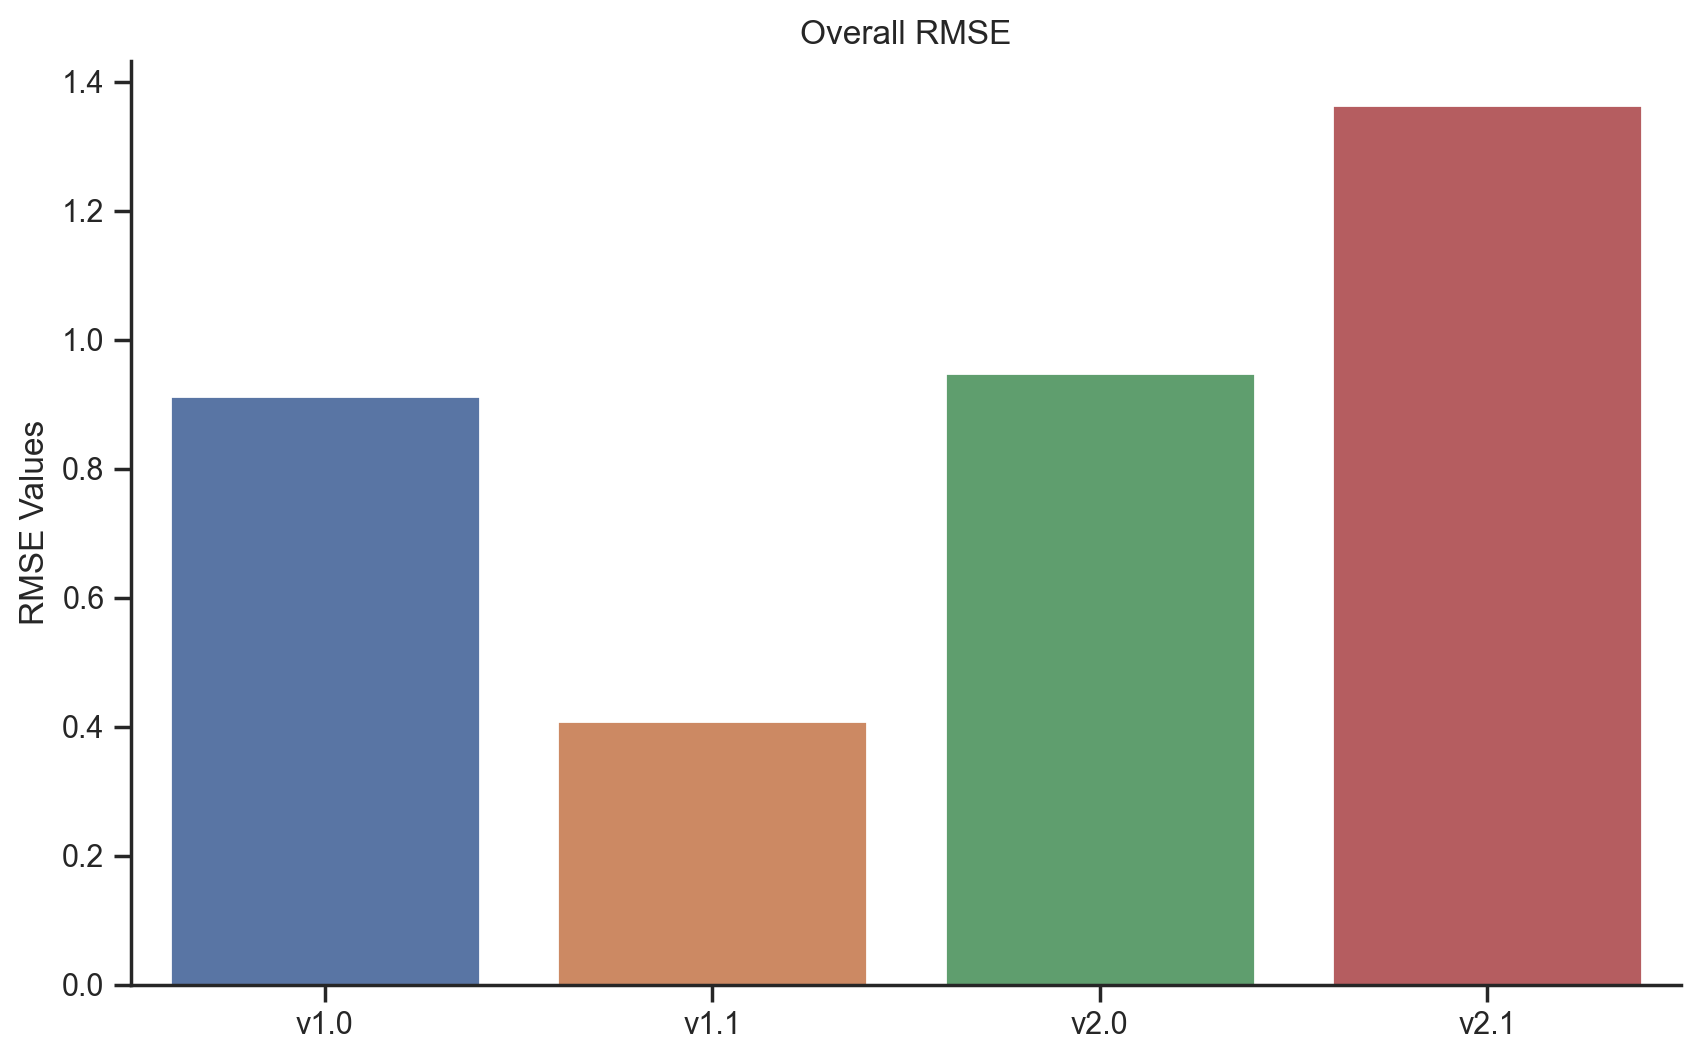
\includegraphics[width=\textwidth]{barplot_overall_score.png}
      \end{figure}
\end{center}
As we can see in the graph, version 1.0 has an RMSE of 0.912. Version 2.0 instead has an RMSE of 0.948. Version 2.1 is the worst one with an RMSE of 1.36. Version 1.1 is the best-performing one with an RMSE of 0.408.
The first approach (1.0) is good in terms of RMSE but not very informative as it only gives a broad evaluation of the operator's communication capabilities, without investigating in detail which are their strengths and weaknesses. The best version in terms of RMSE is 1.1, which also gives a more detailed view of the operator's skills. In the second approach (2.*) the information is more granular, but neither 2.0 nor 2.1 is good enough in terms of RMSE.
\begin{center}
      \begin{figure}
            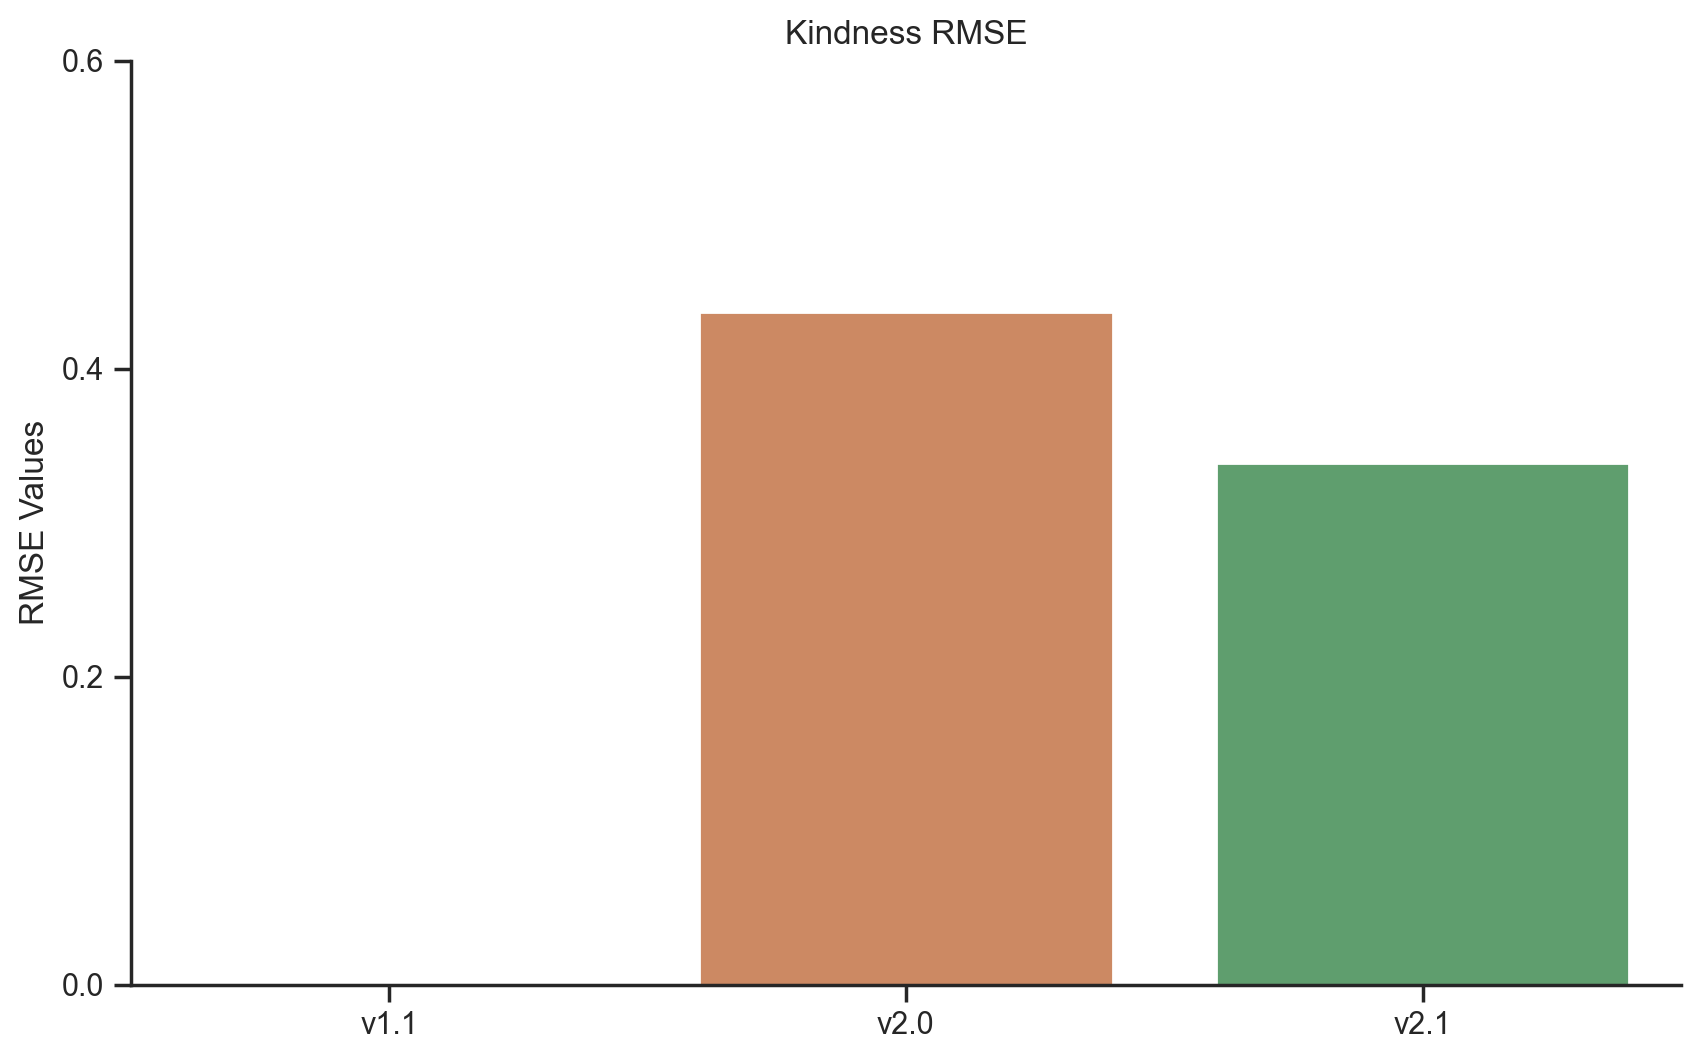
\includegraphics[width=\textwidth]{kindness_score.png}
            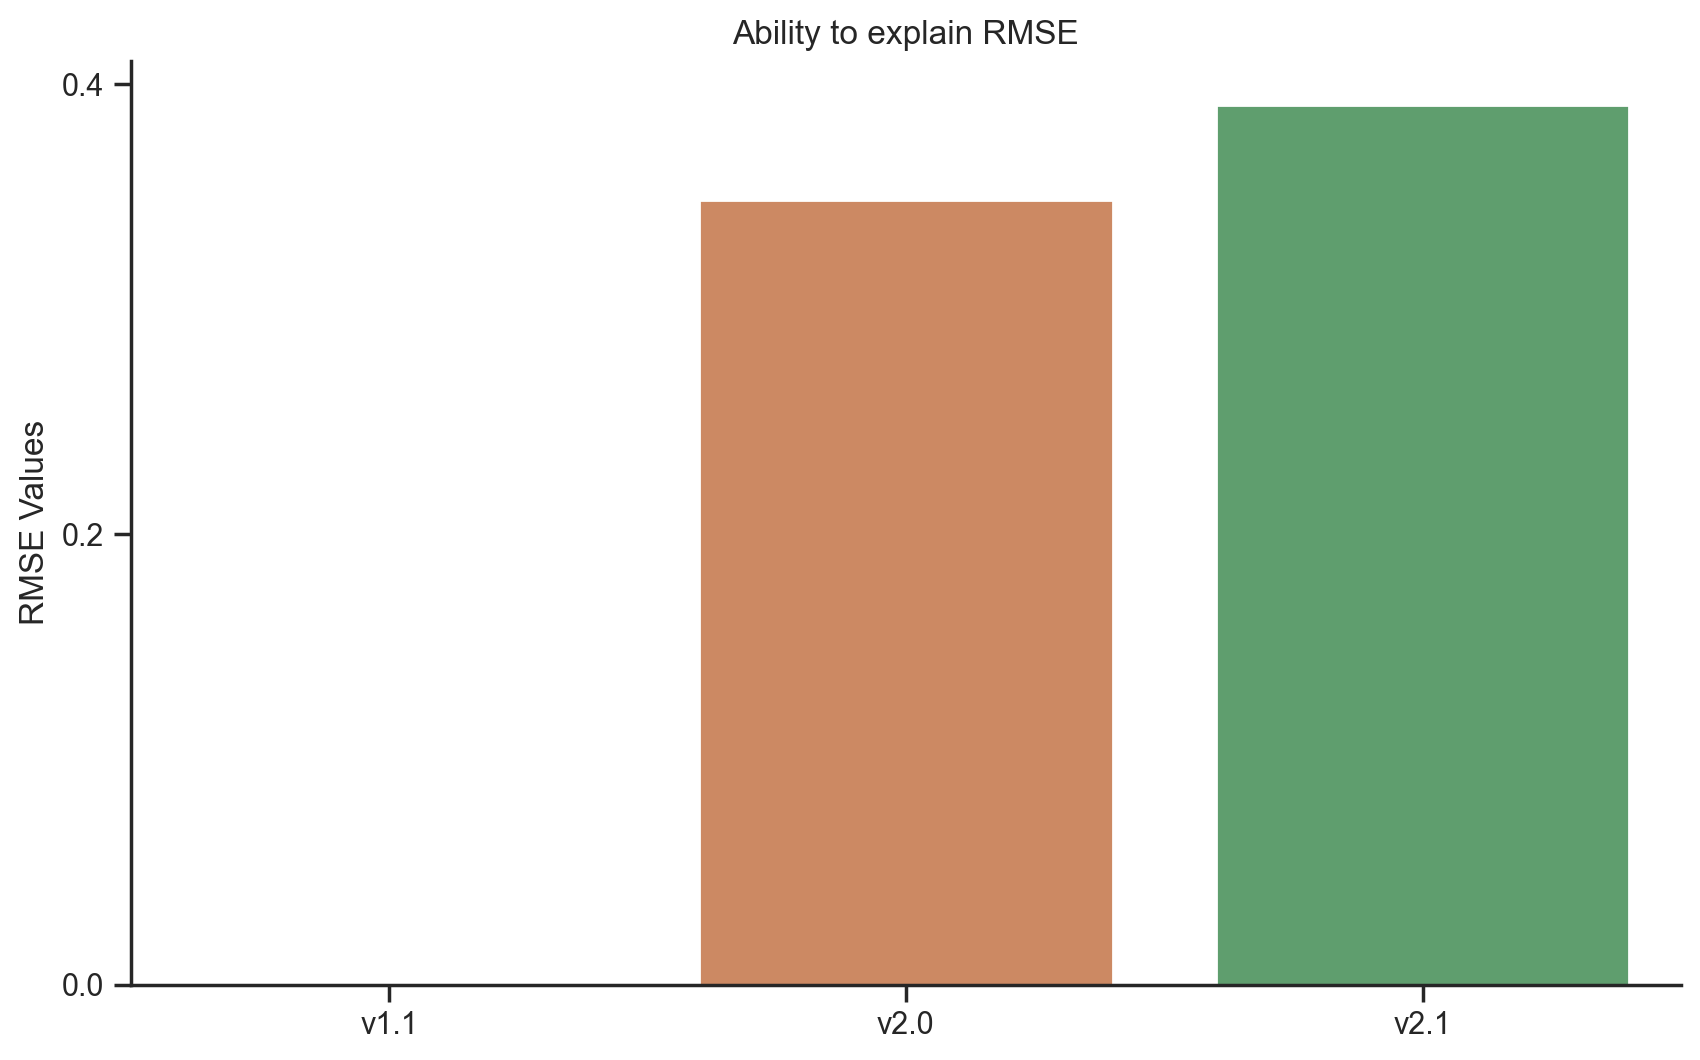
\includegraphics[width=\textwidth]{ate_score.png}
      \end{figure}
      \begin{figure}
            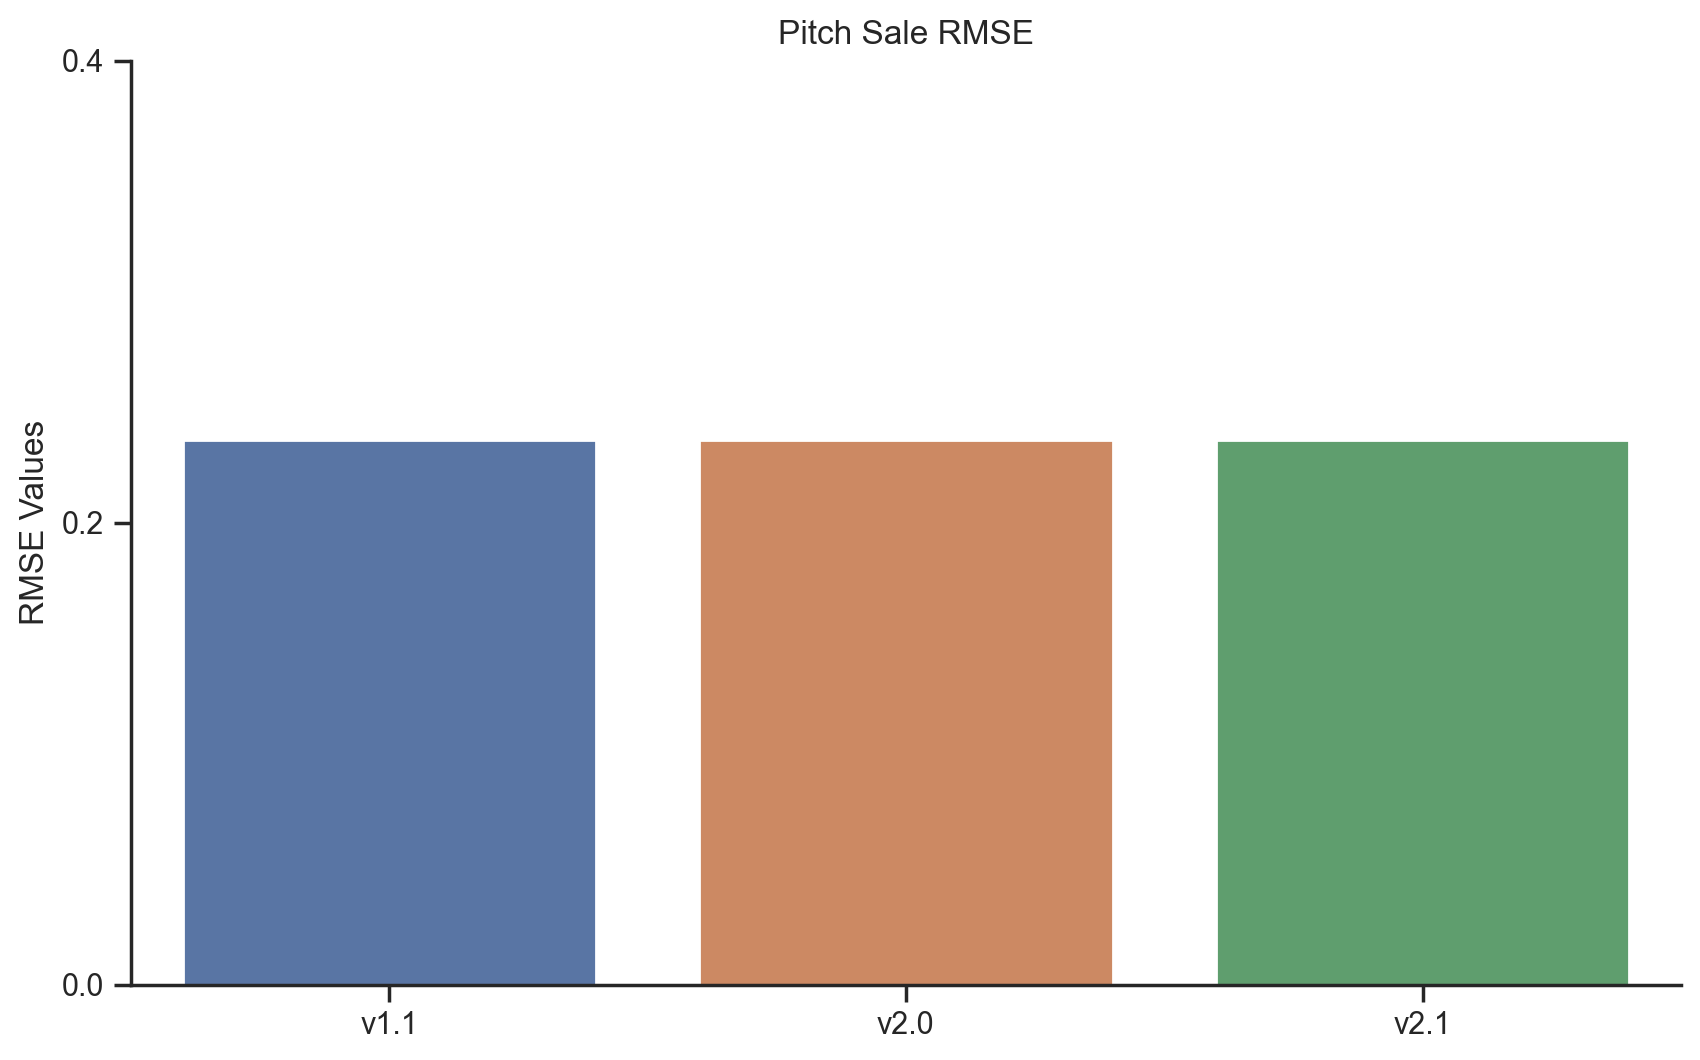
\includegraphics[width=\textwidth]{ps_score.png}
            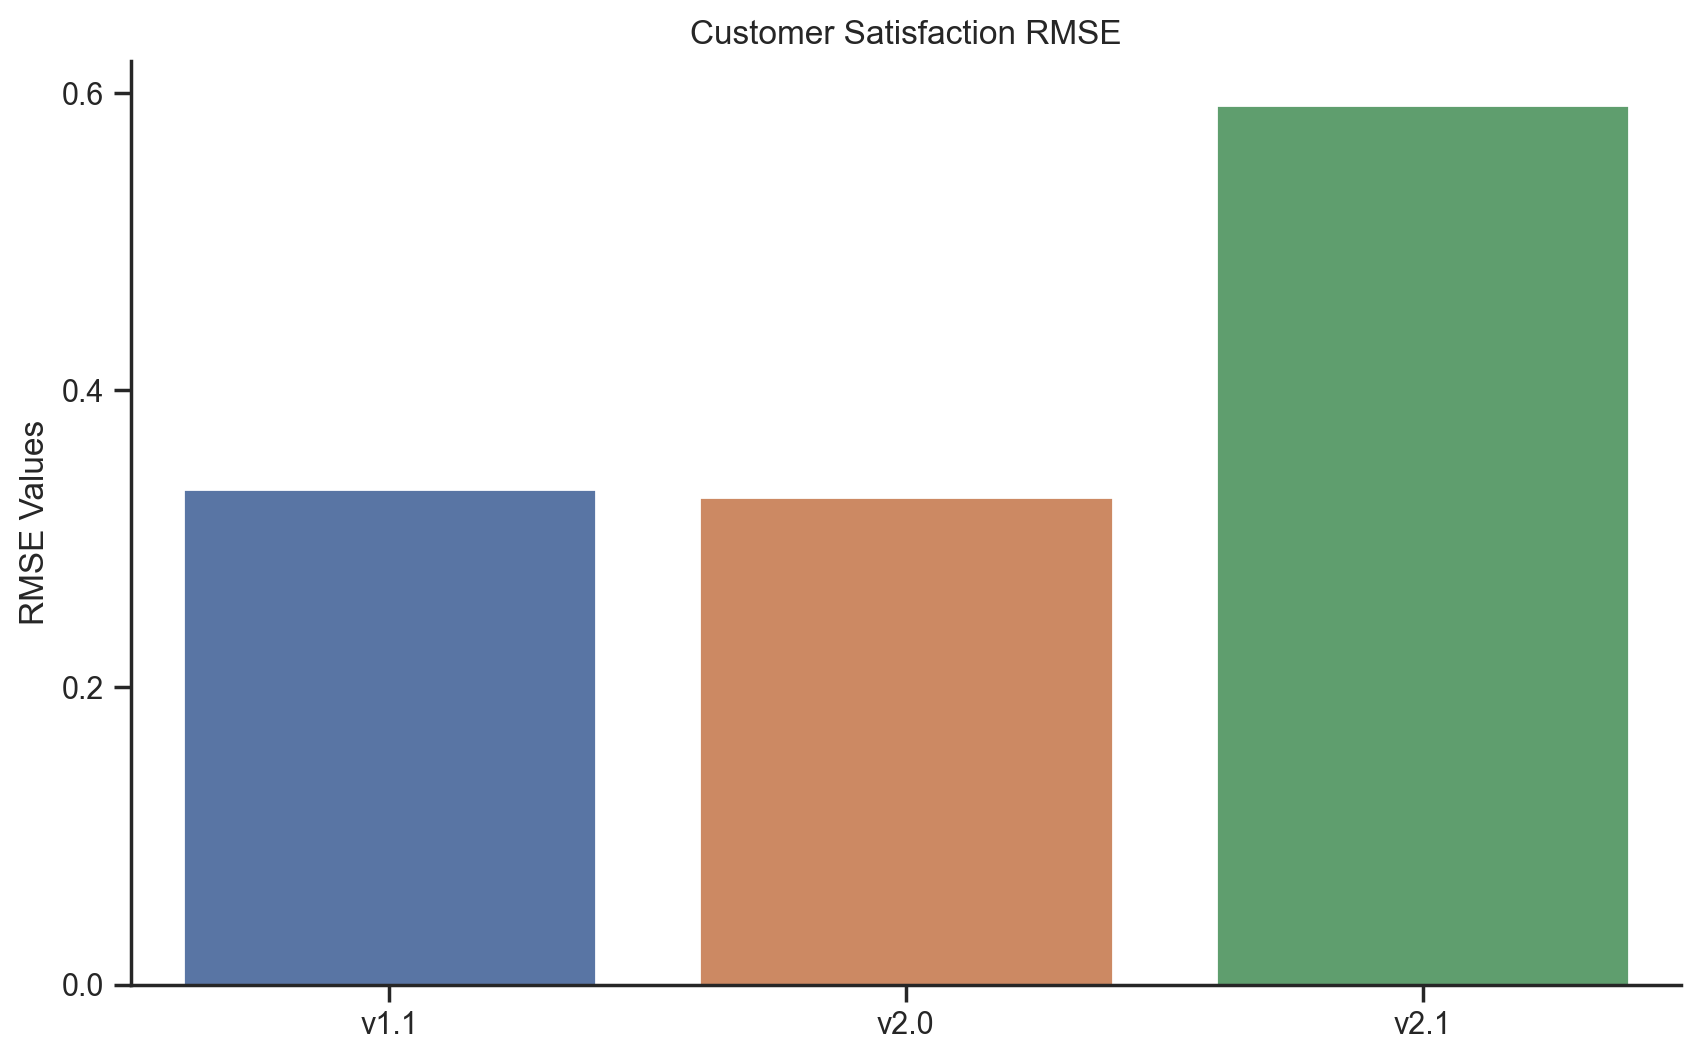
\includegraphics[width=\textwidth]{cs_score.png}
      \end{figure}
\end{center}
As expected, the error on single sub-scores reflects the error on the overall score. It's worth noting that the Pitch Sale sub-score is equal for all the versions evaluating skills separately.
\begin{center}
      \begin{figure}[ht]
            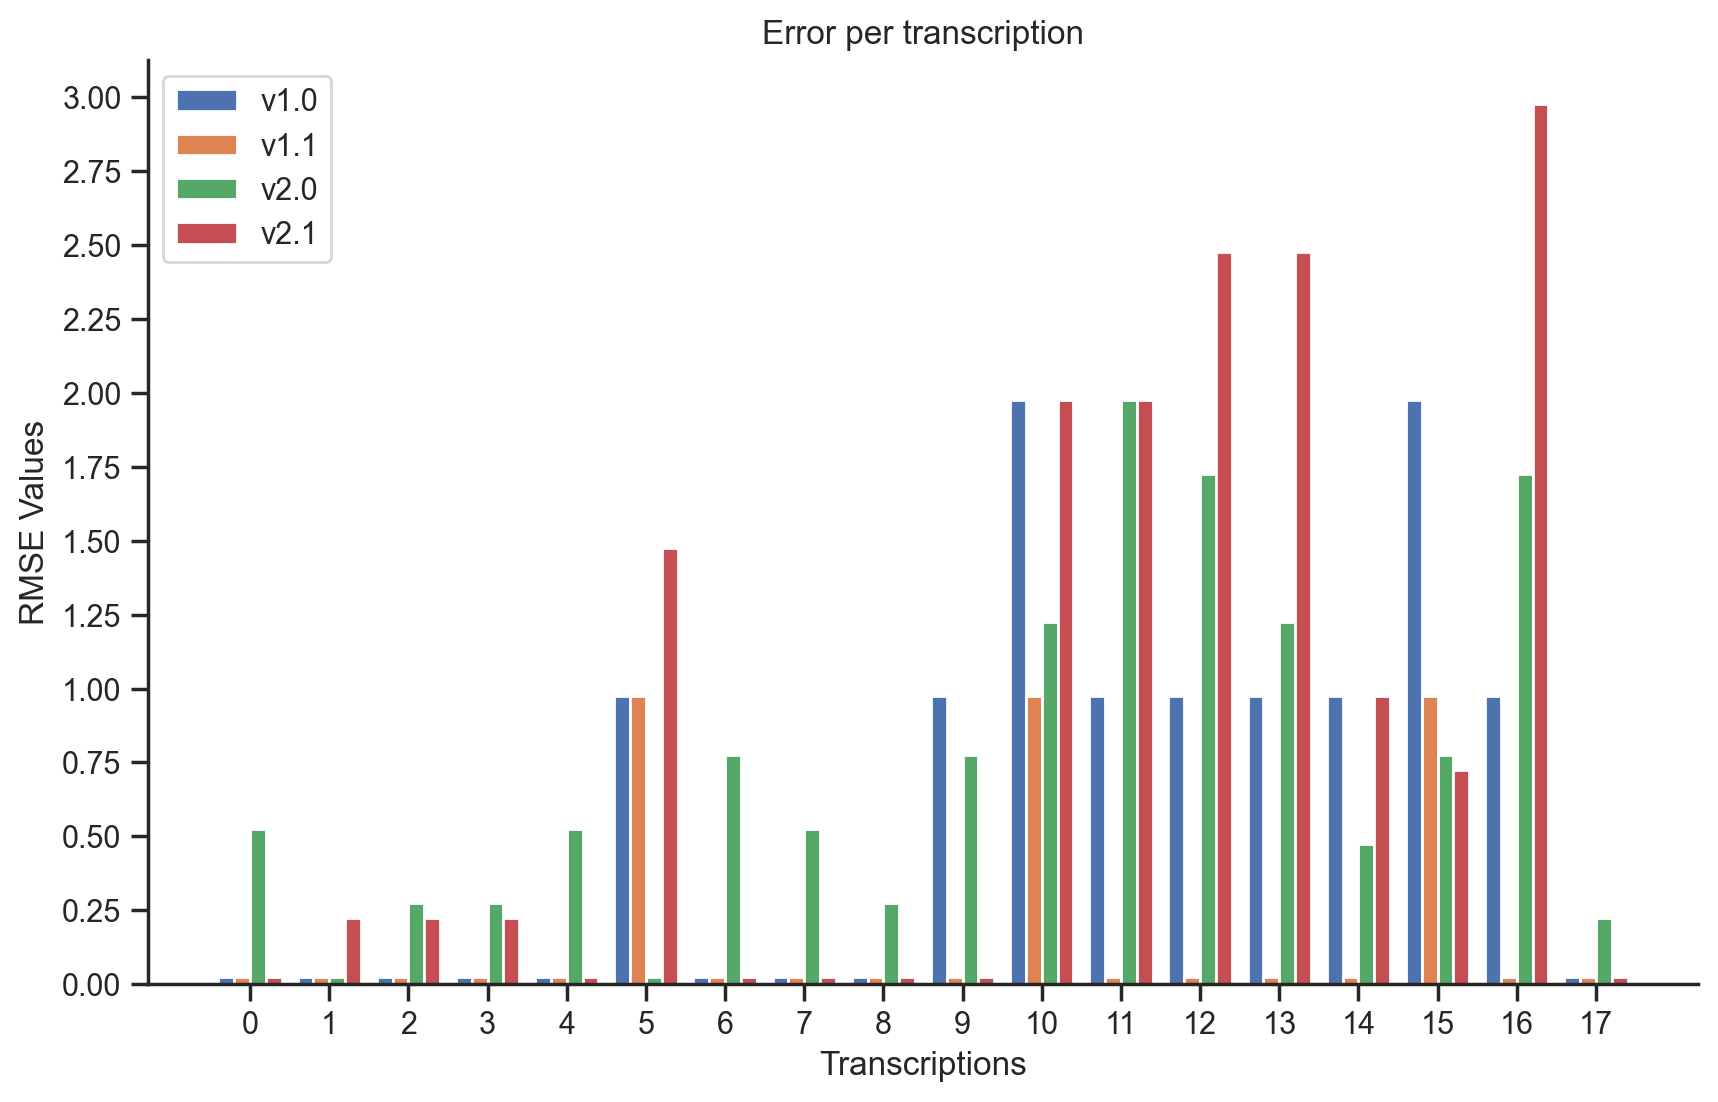
\includegraphics[width=\textwidth]{error_per_transcription.png}
      \end{figure}
\end{center}

It's notable that a significant proportion of errors occur in the additional transcriptions, particularly those that were modified to include instances of unprofessional behavior by the operator. This observation suggests that the introduction of scenarios with unprofessional behavior poses a greater challenge for accurate model performance. It's worth noting that GPT may not be entirely reliable in an automated communication competence mapping context, and caution is warranted when considering its use in a fully automated scoring framework. However, recognizing its potential as a supportive tool for HR purposes is a constructive approach. Leveraging GPT as an assistive tool, rather than relying on it solely for automated decisions, allows human judgment to complement and refine the outputs, contributing to a more nuanced and accurate evaluation process.

\section{Technical Skill Results}

\subsection{Categories and Streets}
The prompt was structured as described before. The following is the version specific question:\\

\textit{Can you identify the category of the ticket and the street in which the problem occurred?}\\

The following are the obtained results:
\begin{center}
      \begin{tabular}{lllrllr}
            \toprule
            \# & CAT       & TCAT      & ICC  & TSTREET       & STREET         & STRSCORE \\
            \midrule
            0  & Disrepair & Disrepair & True & 23rd Street   & 23rd Street    & 100      \\
            1  & Disrepair & Disrepair & True & Atkinson Ave  & W Atkinson Ave & 92       \\
            2  & Disrepair & Disrepair & True & Alvina Ave    & 0              & 0        \\
            3  & Disrepair & Disrepair & True & 0             & 0              & 100      \\
            4  & Disrepair & Disrepair & True & 0             & 0              & 100      \\
            5  & Disrepair & Disrepair & True & 0             & 0              & 100      \\
            6  & Disrepair & Disrepair & True & 0             & 0              & 100      \\
            7  & Disrepair & Disrepair & True & 0             & 0              & 100      \\
            8  & Disrepair & Disrepair & True & 85th Street   & 85th St        & 78       \\
            9  & Disrepair & Disrepair & True & 0             & 0              & 100      \\
            10 & Disrepair & Disrepair & True & 33rd Street   & 33RD ST        & 78       \\
            11 & Disrepair & Disrepair & True & 0             & 0              & 100      \\
            85 & Pothole   & Pothole   & True & 69th Street   & 69th Street    & 100      \\
            86 & Pothole   & Pothole   & True & Rohr Ave      & Rohr Av        & 93       \\
            87 & Pothole   & Pothole   & True & 80th Street   & 80th Street    & 100      \\
            88 & Pothole   & Pothole   & True & 61st Street   & 61st St.       & 74       \\
            90 & Pothole   & Pothole   & True & mason Street  & E Mason Street & 92       \\
            91 & Pothole   & Pothole   & True & 40th Street   & N. 40th St.    & 80       \\
            92 & Pothole   & Pothole   & True & Howard Ave    & E Howard Ave   & 91       \\
            93 & Pothole   & Pothole   & True & Harbor Street & Harbor Street  & 100      \\
            \bottomrule
      \end{tabular}
\end{center}

\subsection{Subcategories}
The prompt was structured as described before. The following is the version specific question:\\

\textit{The problems are related to previously identified category. Can you identify the ticket subcategory?}\\

The following are the obtained results:
\begin{center}
      \begin{tabular}{lllr}
            \toprule
            \# & SUBC                     & TSUBC                    & ISC   \\
            \midrule
            0  & Garbage Cart: Additional & Garbage Cart: Additional & True  \\
            1  & Garbage Cart: Additional & Garbage Cart: Additional & True  \\
            2  & Garbage Cart: Additional & Garbage Cart: Additional & True  \\
            3  & Garbage Cart: Missing    & Garbage Cart: Additional & False \\
            4  & Garbage Cart: Additional & Garbage Cart: Additional & True  \\
            5  & Garbage Cart: Additional & Garbage Cart: Additional & True  \\
            6  & Garbage Cart: Damaged    & Garbage Cart: Additional & False \\
            7  & Garbage Cart: Additional & Garbage Cart: Additional & True  \\
            8  & Garbage Cart: Damaged    & Garbage Cart: Additional & False \\
            9  & Garbage Cart: Additional & Garbage Cart: Additional & True  \\
            10 & Garbage Cart: Additional & Garbage Cart: Additional & True  \\
            11 & Garbage Cart: Additional & Garbage Cart: Additional & True  \\
            12 & Garbage Cart: Additional & Garbage Cart: Additional & True  \\
            13 & Garbage Cart: Additional & Garbage Cart: Additional & True  \\
            14 & Garbage Cart: Additional & Garbage Cart: Additional & True  \\
            15 & Garbage Cart: Additional & Garbage Cart: Additional & True  \\
            16 & Garbage Cart: Additional & Garbage Cart: Additional & True  \\
            17 & Garbage Cart: Missing    & Garbage Cart: Additional & False \\
            18 & Garbage Cart: Additional & Garbage Cart: Additional & True  \\
            19 & Garbage Cart: Additional & Garbage Cart: Additional & True  \\
            20 & Garbage Cart: Additional & Garbage Cart: Additional & True  \\
            \bottomrule
      \end{tabular}
\end{center}

\subsection{Technical results comparison}
The overall accuracy for both the category and subcategory extraction is similar and around 80\%.
\begin{center}
      \begin{figure}[ht]
            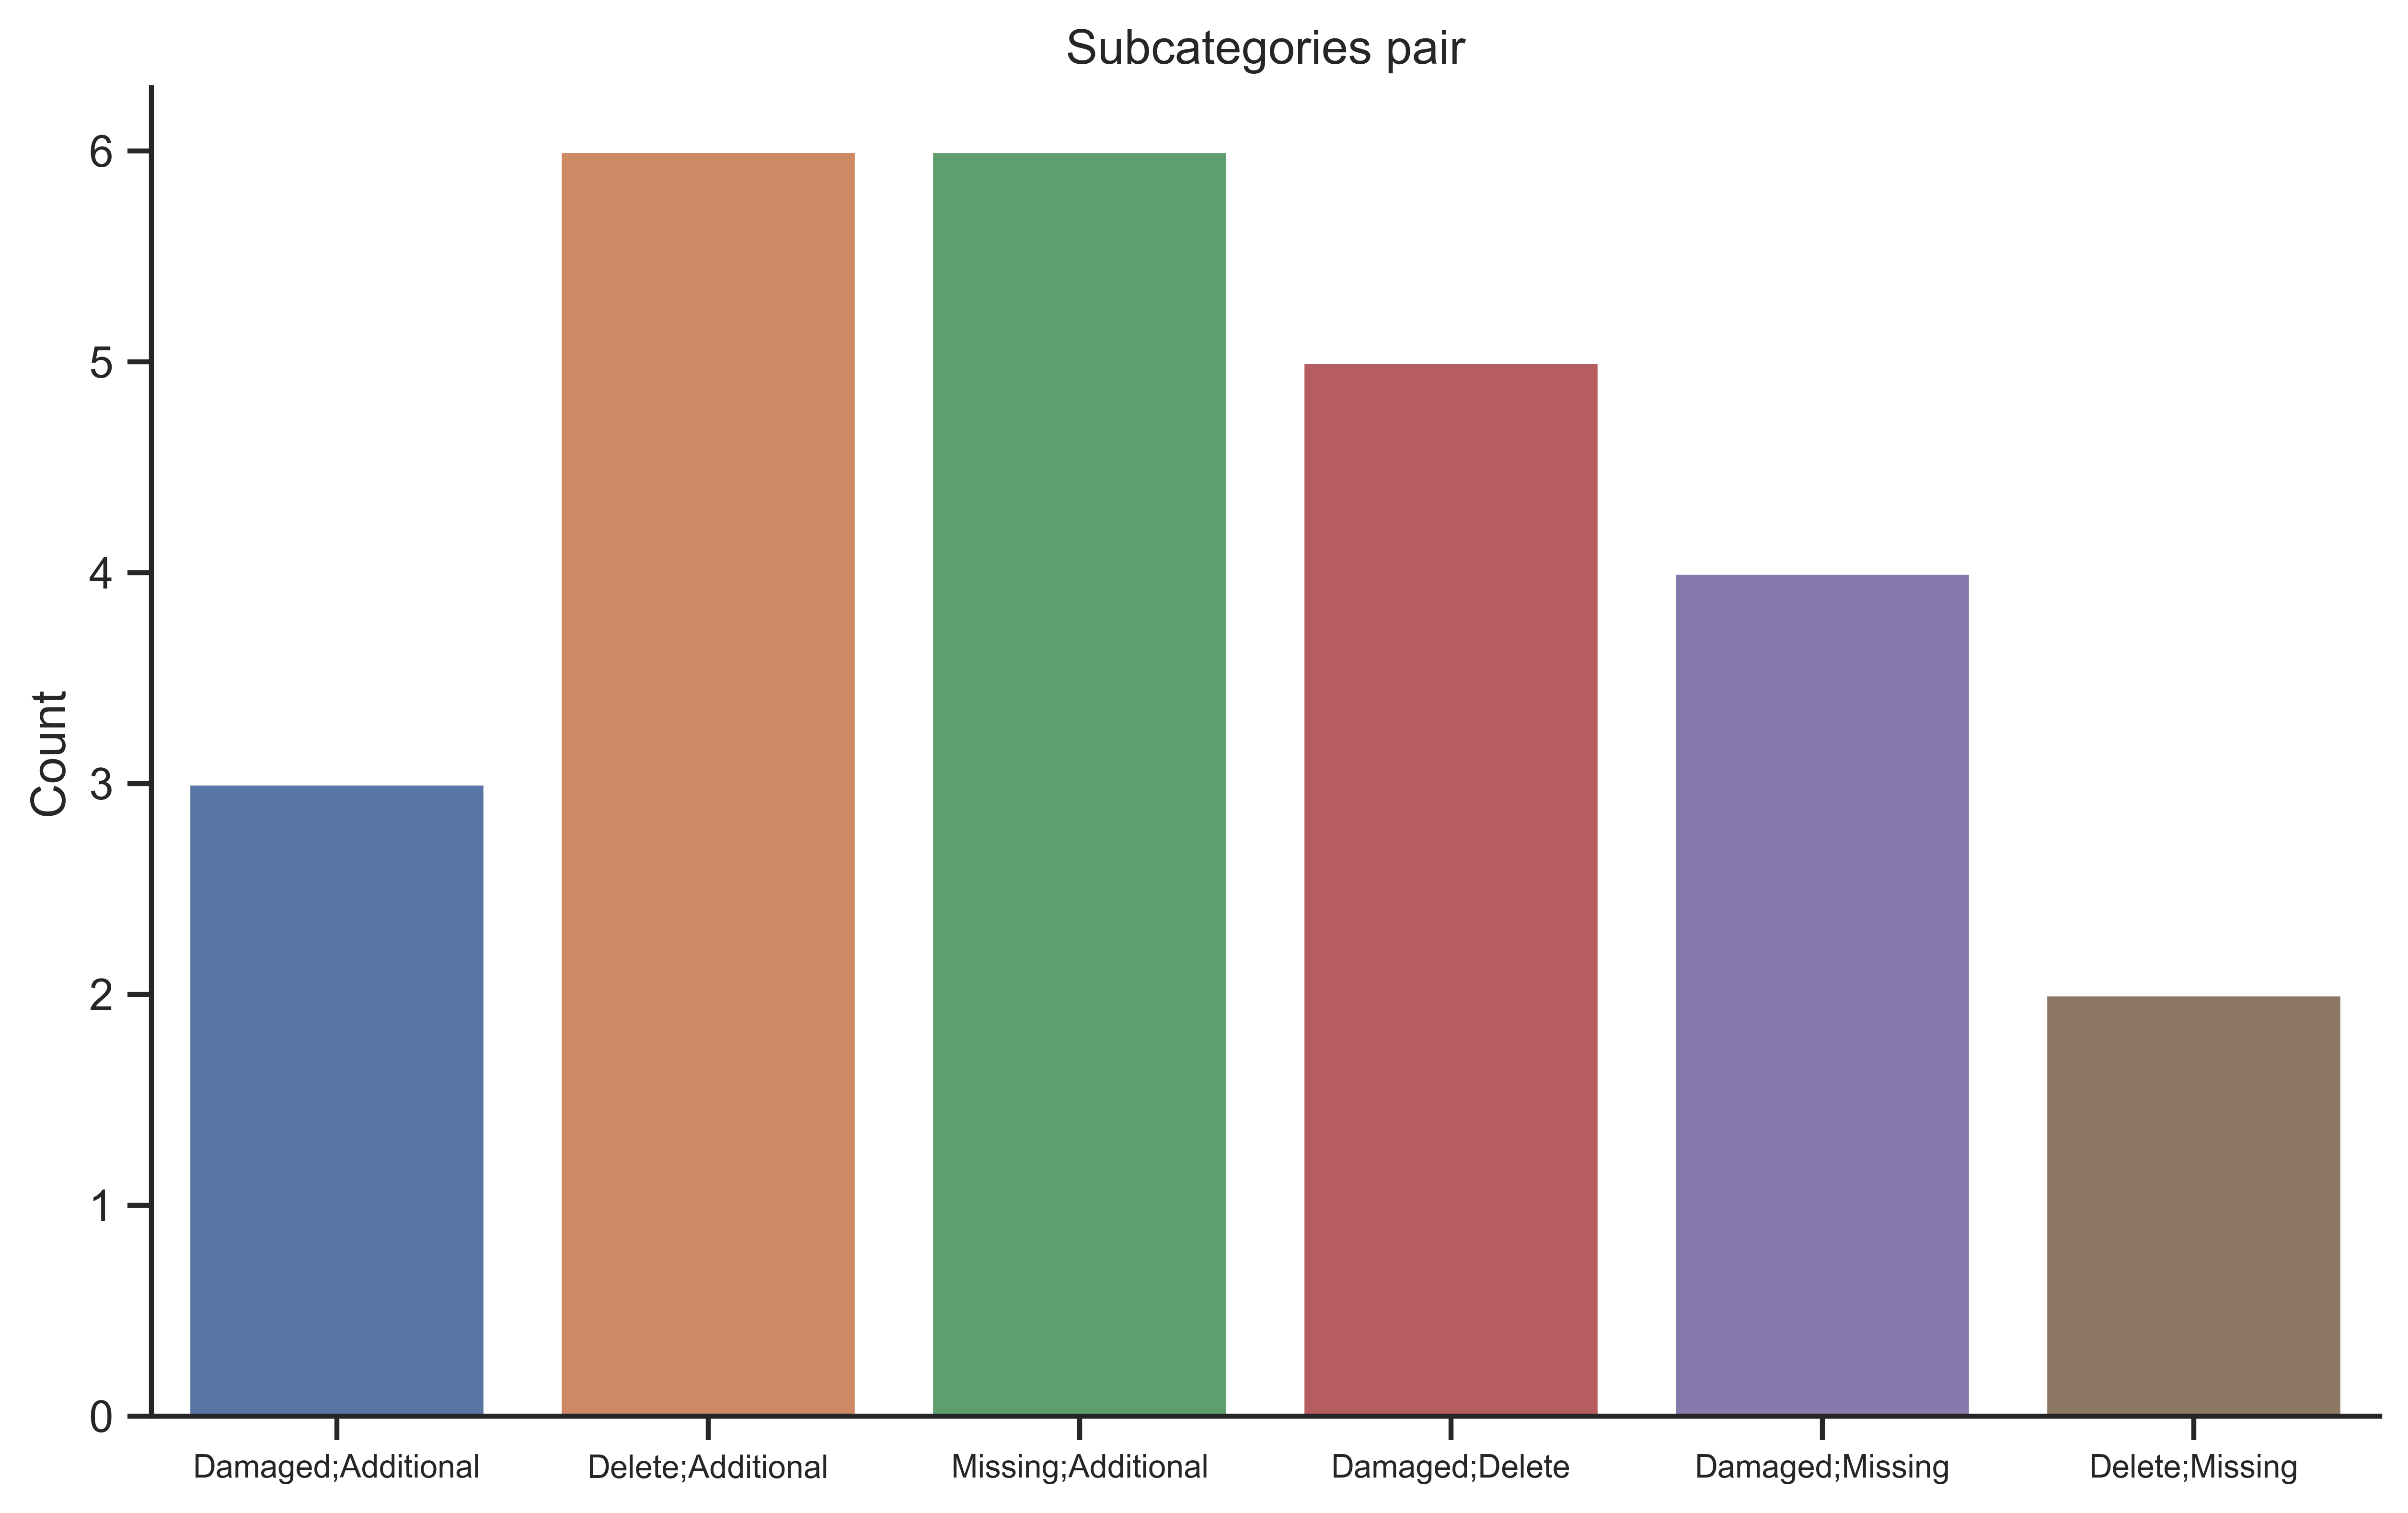
\includegraphics[width=\textwidth]{subcategory_pairs.png}
      \end{figure}
\end{center}
As we can see in most misclassification cases the "Garbage Collection: Additional Cart" is present. Specifically, the two most misclassified pairs are "Garbage Collection: Delete Cart" which is identified as "Garbage Collection: Additional Cart" and "Garbage Collection: Missing Cart" which is identified as "Garbage Collection: Additional Cart". The confusion is due to the strong similarity between subcategories: eg. an additional cart request could be due to a missing cart or a damaged cart, which means it's not necessarily easy to understand the correct category both for humans and GPT. We also hypothesized that sometimes there could be multiple correct categories.
\begin{center}
      \begin{figure}[ht]
            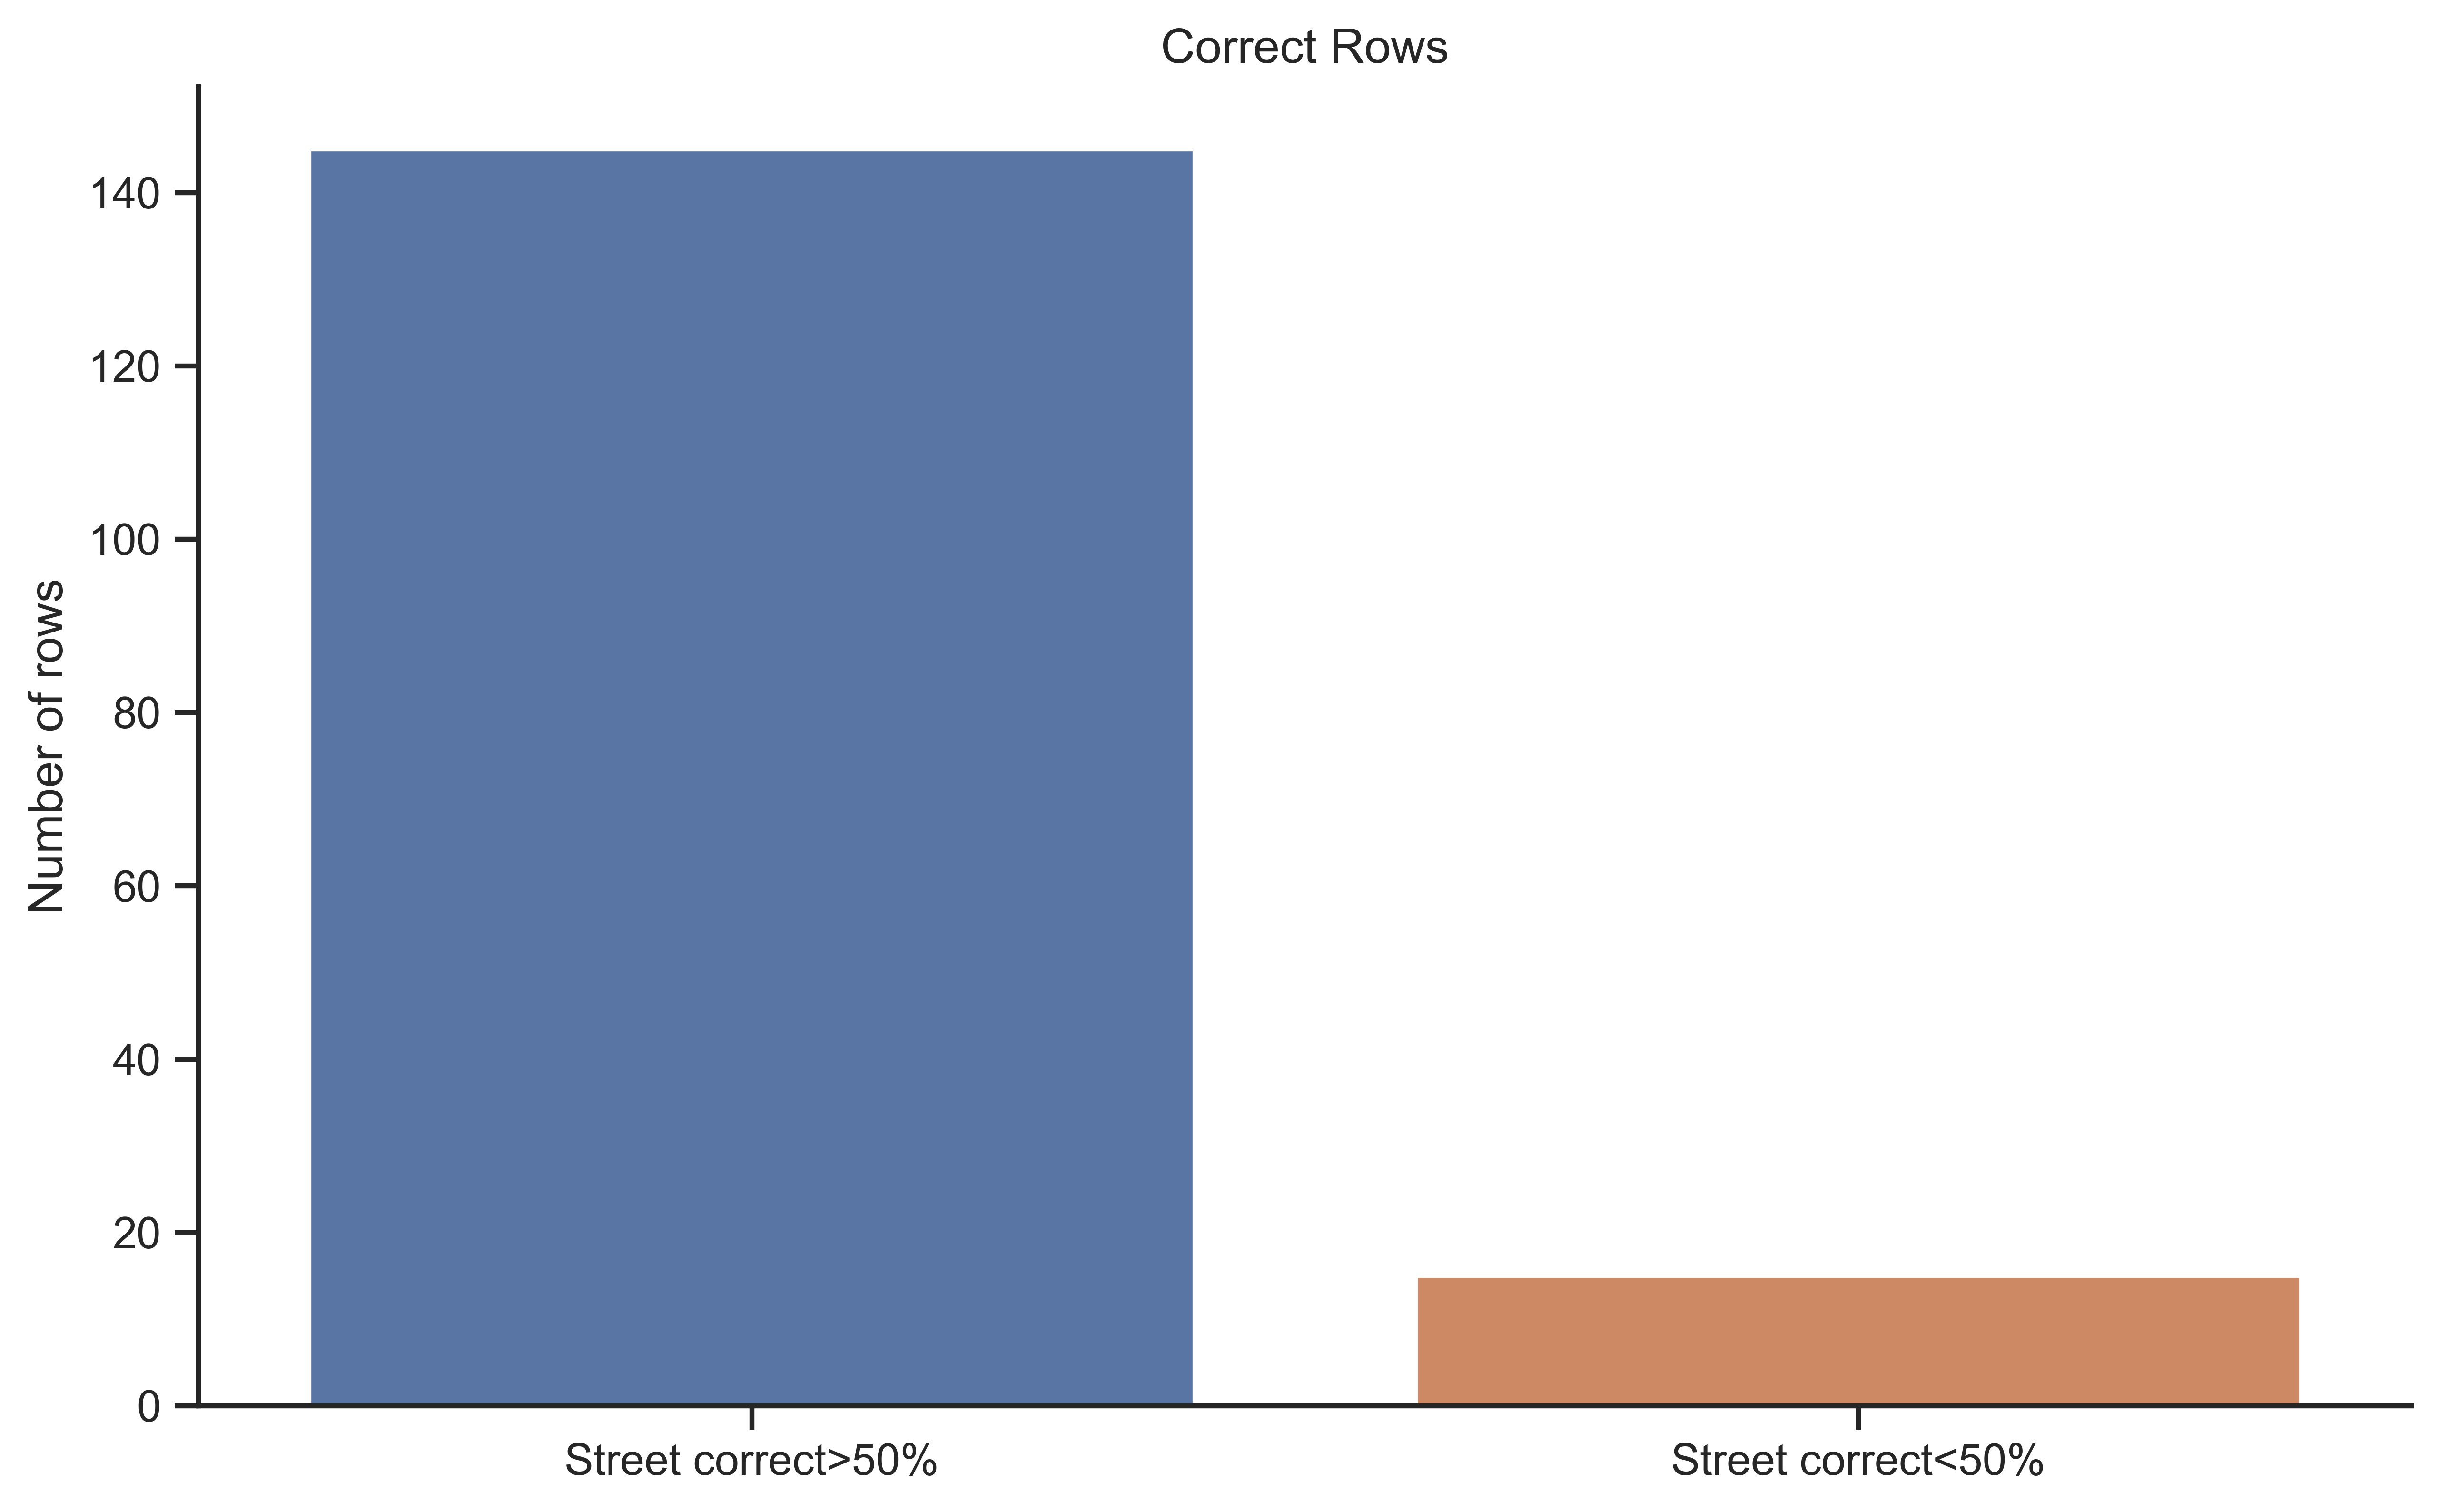
\includegraphics[width=0.99\textwidth]{street_recognition.png}
      \end{figure}
\end{center}
To evaluate the ability of the model to recognize the location in which the ticket request is taking place, we compared GPT's answer with a manually extracted label using the Python package fuzzywuzzy as specified in \ref{sec:techcomp}. This package gives a score from 0 to 100 based on how similar a certain string is with respect to the target string.
In most cases, GPT was able to find the correct street or set of streets, even if sometimes it wasn't able to infer the street type (Street, Avenue, Boulevard). In 90\% of cases, the correctness of the produced string was higher than 50/100. In most cases the string is classified with a score of 100, meaning the model is usually able to identify the street.
\begin{center}
      \begin{figure}[ht]
            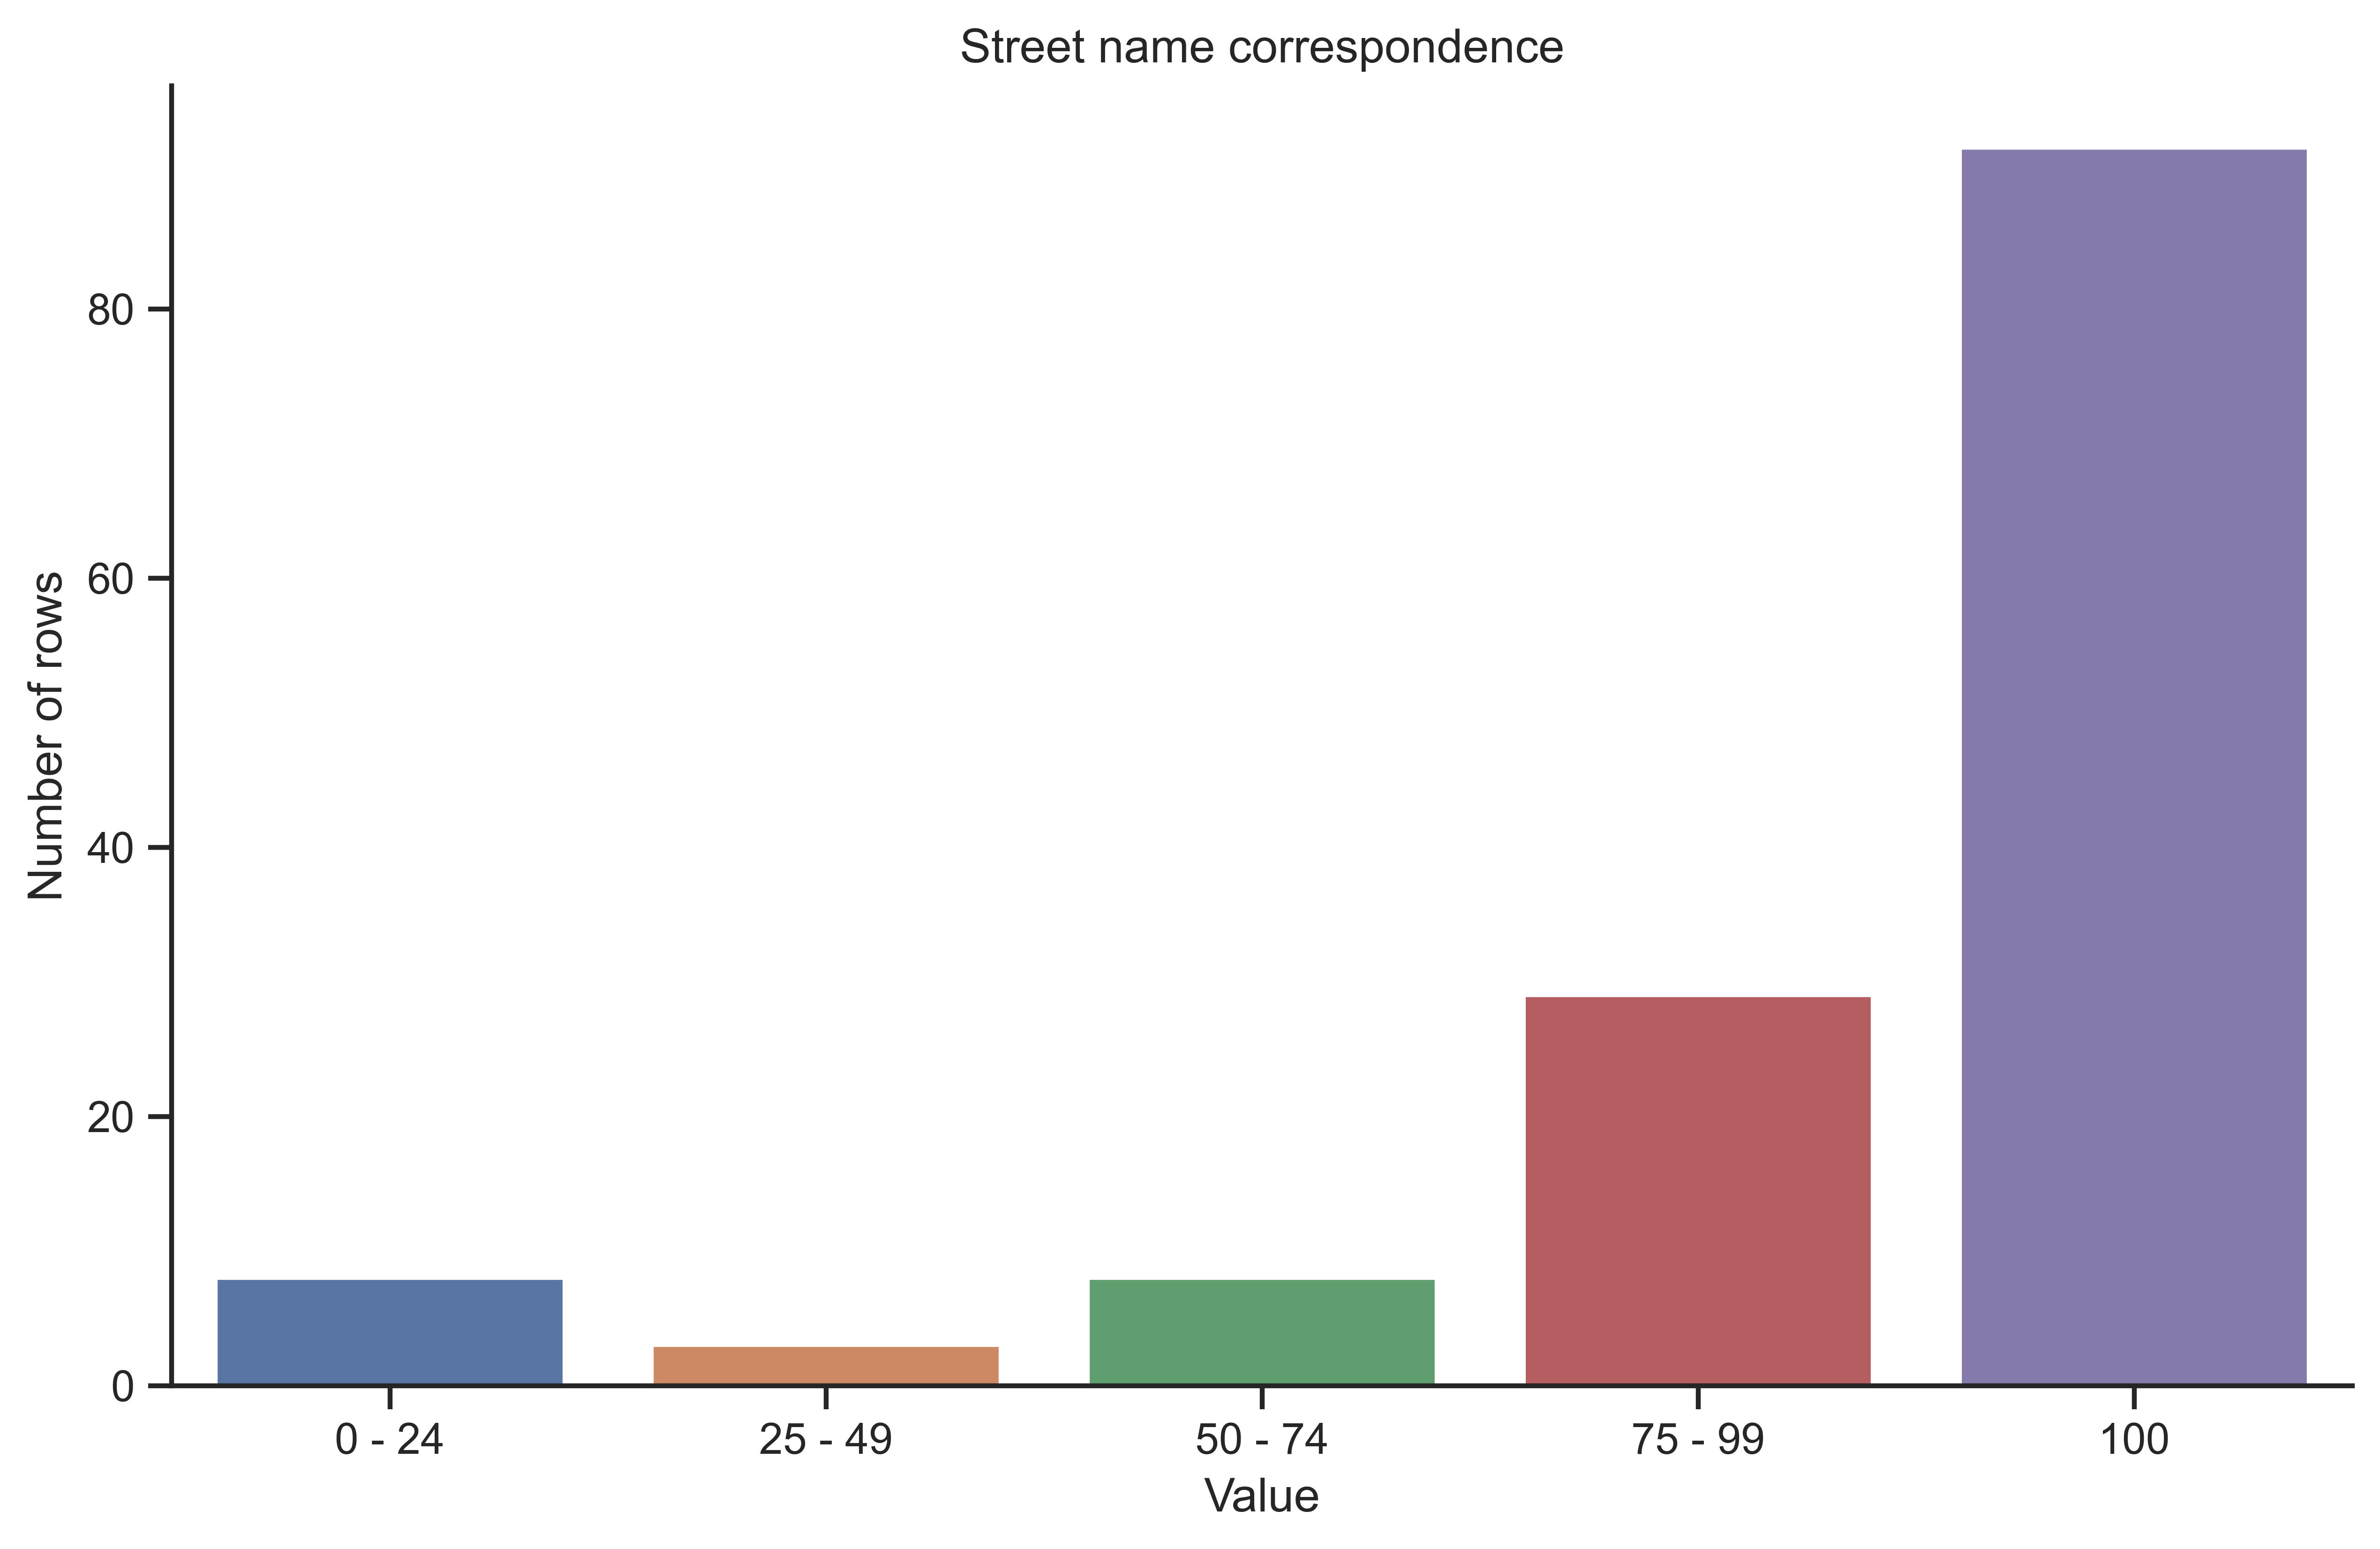
\includegraphics[width=0.99\textwidth]{street_correctness.png}
      \end{figure}
\end{center}

\newpage
\section{Problem Management Results}
\label{sec:probmanageres}
The prompt was structured as described before. The following are the questions:\\

\textit{Did the operator seem professional to you?                                                                                                          \\
      Is the number of days it took to resolve the problem greater than 2?                                                                                        \\
      Has the customer been updated on the ticket situation?                                                                                                      \\
      Has the technician found that the problem is attributable to the internal system (e.g. problems with the router or configurations) or to the external line? \\
      Was it necessary to involve the local technician externally?                                                                                                \\
      While resolving the issue, was it necessary to replace/change the router?                                                                                   \\
      Was the replaced router actually broken/faulty?}\\

The following are the obtained results:
\begin{center}
      \begin{tabular}{ccccccccccccccc}
            \toprule
            \# & Q1 & T\_Q1 & Q2 & T\_Q2 & Q3 & T\_Q3 & Q4 & T\_Q4 & Q5 & T\_Q5 & Q6 & T\_Q6 & Q7 & T\_Q7 \\
            \midrule
            1  & 1  & 1     & -1 & -1    & 1  & 1     & 0  & 0     & 2  & 2     & 0  & 0     & 0  & 0     \\
            2  & 1  & 1     & -1 & -1    & 1  & 1     & 1  & 1     & -2 & -2    & 0  & 0     & 0  & 0     \\
            3  & 1  & 1     & -1 & 1     & 1  & 1     & 1  & 1     & 2  & 2     & 1  & 1     & 1  & 1     \\
            4  & 1  & 1     & -1 & 1     & 1  & 1     & 1  & 1     & 2  & 2     & 0  & 0     & 0  & 0     \\
            5  & 1  & 1     & -1 & 1     & 1  & 1     & 0  & 0     & 2  & 2     & 0  & 0     & 0  & 0     \\
            6  & 1  & 1     & -1 & 1     & 1  & 1     & 0  & 0     & 2  & 2     & 0  & 0     & 0  & 0     \\
            7  & 1  & 1     & -1 & -1    & 1  & 1     & 1  & 1     & -2 & -2    & 1  & 1     & 1  & 1     \\
            8  & 1  & 1     & -1 & 1     & 1  & 1     & 1  & 1     & 2  & 2     & 0  & 0     & 0  & 0     \\
            9  & 1  & 1     & -1 & 1     & 1  & 1     & 0  & 0     & 2  & 2     & 0  & 0     & 0  & 0     \\
            10 & 1  & 1     & -1 & -1    & 1  & 1     & 1  & 1     & -2 & -2    & 1  & 1     & 1  & 1     \\
            \bottomrule
      \end{tabular}
\end{center}


\subsection{Problem management results comparison}

We choose RMSE to measure the error between GPT values and the expected ones, as this measure works well with regression problems. On the x-axis, we have the questions, while on the y-axis there are the RMSE values. The accuracy reached 90\%. As we can see, GPT always answers correctly to six out of seven questions; the only wrong one is the second question, which is about the overall ticket time resolution. This issue isn't hard to solve since the ticket-solving duration can be easily retrieved from the AEM Fiber system, as the domain expert suggested.

\chapter{List of Abbreviations}

\begin{description}
      \item[KIND:] Kindness
      \item[EXP:] Ability to explain themselves
      \item[SALE:] Initiative of the operator to make a pitch sale
      \item[SAT:] Customer satisfaction
      \item[TKIND:] Target Kindness
      \item[TEXP:] Target ability to explain themselves
      \item[TSALE:] Target initiative of the operator to make a pitch sale
      \item[TSAT:] Target customer satisfaction
      \item[OV:] Overall
      \item[TOV:] Target Overall
      \item[DIFF:] Difference between OV and TOV
      \item[CAT:] Category
      \item[TCAT:] Target Category
      \item[ICC:] Is Category Correct
      \item[STREET:] Street
      \item[TSTREET:] Target Street
      \item[STRSCORE:] Street Score
      \item[SUBC:] Subcategory
      \item[TSUBC:] Target Subcategory
      \item[ISC:] Is Subcategory Correct
      \item[Q\#:] Answer to question number \#
      \item[T\_Q\#:] Target answer to question number \#
\end{description}